


% About StagYY


\begin{frame}{StagYY}

  \begin{block}{About StagYY}
  \begin{itemize}
   \item Mantle convection solver
   \item Cartesian, 3D spherical shell, cylindrical domains
   \item Further details: P.~Tackley, J. PEPI (2008)
  \end{itemize}
  \end{block}

  \begin{block}{Discretization and Solver}
  \begin{itemize}
   \item Staggered differences finite volume method
   \item Multigrid solver (V- or F-cycles)
   \item Matrix-free residual evaluation and relaxation
  \end{itemize}
  \end{block}

\end{frame}


% Anatomy of a Residual/relaxation step

\begin{frame}{StagYY}

  \begin{block}{Conservation Equations}
         \vspace*{-0.5cm}
        \begin{align*}
          \nabla \cdot (\rho \vector v) &= 0  & & \mathrm{(mass)} \\
          \nabla \cdot \vector \sigma  - \nabla p &=  \frac{\mathrm{Ra}.\vector r \rho(C,r,T)}{\Delta  \rho_{\mathrm{thermal}}} & & \mathrm{(momentum)} \\
          \rho  C_{\mathrm p} \frac{\partial T}{\partial t} &= - \mathrm{Di}_{\mathrm s} \alpha \rho T v_r + \nabla \cdot (k \nabla T) + \rho H + \frac{\mathrm{Di}_{\mathrm s}}{\mathrm{Ra}} \vector \sigma : \vector \varepsilon  & & \mathrm{(energy)} 
         \end{align*}
  \end{block}

  %\pause
  \begin{center}
   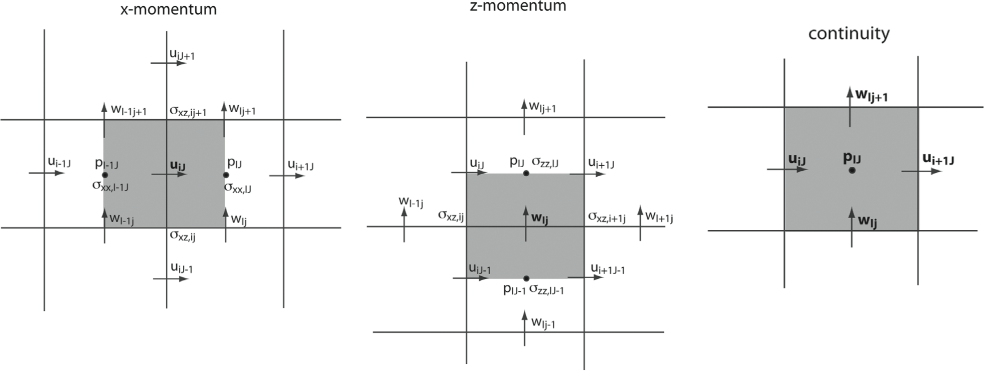
\includegraphics[width=0.7\textwidth]{figures/stagyy-discretization} \\
   {\scriptsize (P.~Tackley, Stagyy User Manual)}
  \end{center}

\end{frame}

\begin{frame}[fragile]\frametitle{StagYY: Performance Modeling}

{ \footnotesize
\begin{minipage}{0.45\textwidth}
\begin{block}{Iterated relaxation}
\begin{verbatim}
 - Update z-component of velocity
 - Exchange values of vz at boundaries
 
 - Compute pressure correction
 - Exchange correction values at boundaries
 - Apply pressure correction
 - Update velocity based on new pressure
 - Exchange boundary pressure and velocity
 
 - Update y-component of velocity
 - Exchange values of vy at boundaries

 - Update x-component of velocity
 - Exchange values of vx at boundaries
\end{verbatim}
\end{block}
\end{minipage}
\begin{minipage}{0.45\textwidth}
\begin{block}{All moments simultaneously}
\begin{verbatim}
 - Compute updates for all velocity components
 - Exchange boundary pressure and velocity

 - Compute correction for pressure p
 - Exchange correction values at boundaries
 - Apply pressure correction
 - Update velocity based  on new pressure
 - Exchange boundary pressure and velocity
   
   
   
   
  
   
\end{verbatim}
\end{block}
\end{minipage}
}


\end{frame}

% Optimization of boundary gather/scatter

\begin{frame}{StagYY}

  \begin{block}{GPU Data Handling}
  \begin{itemize}
   \item Fields on each multigrid hierarchy reside on GPU
   \item Stack-like mechanism for resident GPU data
  \end{itemize}
  \end{block}

  %\pause
  \begin{block}{GPU Boundary Value Handling}
  \begin{itemize}
   \item pTatin3d results: Pay attention to this
   \item MPI-like \texttt{gather} and \texttt{scatter} implemented
  \end{itemize}
  \end{block}

\begin{flushright}
  %\only<3>{ \vspace*{-4cm} \includegraphics[width=0.305\textwidth]{figures/gather} }
  %\only<4>{ \vspace*{-4cm} \includegraphics[width=0.305\textwidth]{figures/scatter} }
  \vspace*{-4cm} \includegraphics[width=0.305\textwidth]{figures/scatter}
\end{flushright}
  
\end{frame}





% Results (compare to CPU)

\begin{frame}{StagYY}

  \begin{block}{GPU Acceleration}
  \begin{itemize}
   \item One thread per residual entry
   \item Common kernel code path for CUDA and OpenCL
  \end{itemize}
  \end{block}

  %\pause
  \begin{block}{Observations}
   \begin{itemize}
    \item It works!
    %\pause
    \item Kernels fairly fast out-of-the-box!
   \end{itemize}
  \end{block}
  
\begin{center}
\begin{tabular}{|r|c|c|c|c|c|}
 \hline
 \textbf{nxtot=nytot=nztot}   & \textbf{GPU, CUDA, xyz} & \textbf{GPU, CUDA, classic}  &\textbf{Sequential} & \textbf{8 MPI ranks}  \\
 \hline
 \hline
 32                           &  0.27 &   0.28  &     0.36    &  0.08  \\
 64                           &  1.21 &   1.39  &     3.04    &  0.50  \\
 128                          &  5.66 &   5.33  &    24.4     &  4.4  \\
 256                          &  38.4 &  25.7   &    timeout  & 36.1  \\
 \hline
\end{tabular} \\
(Timings in seconds, Piz Daint after upgrade)
\end{center}
  
\end{frame}



% Profiling: Communication overhead!

\begin{frame}[fragile]\frametitle{StagYY: Performance Modeling}

  \begin{block}{GPU Profiling}
   \begin{itemize}
    \item 60-65 percent of GPU-time spent on PCI-Express transfer
    \item Checked: No unnecessary transfers, full bandwidth, etc.
   \end{itemize}
  \end{block}

  \begin{center}
\begin{tabular}{|r|c|c|c|c|}
 \hline
 \textbf{nxtot=nytot=nztot}   & \textbf{GPU, CUDA, xyz} & \textbf{GPU, CUDA, classic}  \\
 \hline
 \hline
 CUDA memcpy HtoD           &  39.03\% &  49.98\%  \\
 CUDA memcpy DtoH           &  20.78\% &  16.03\%  \\
 \hline
\end{tabular}
\end{center}


\end{frame}


%
% Performance Model: Figure out the problem
%
\begin{frame}[fragile]
\frametitle{StagYY: Performance Modeling}
  \begin{block}{Pitfall: GPUs are too fast for PCI-Express}
  \begin{itemize}
   \item Latest GPU peaks: 720 GB/sec from GPU-RAM, 16 GB/sec for PCI-Express
   \item 40x imbalance (!)
  \end{itemize}
  \end{block}

  %\pause
  \begin{center} \vspace*{-0.8cm}
    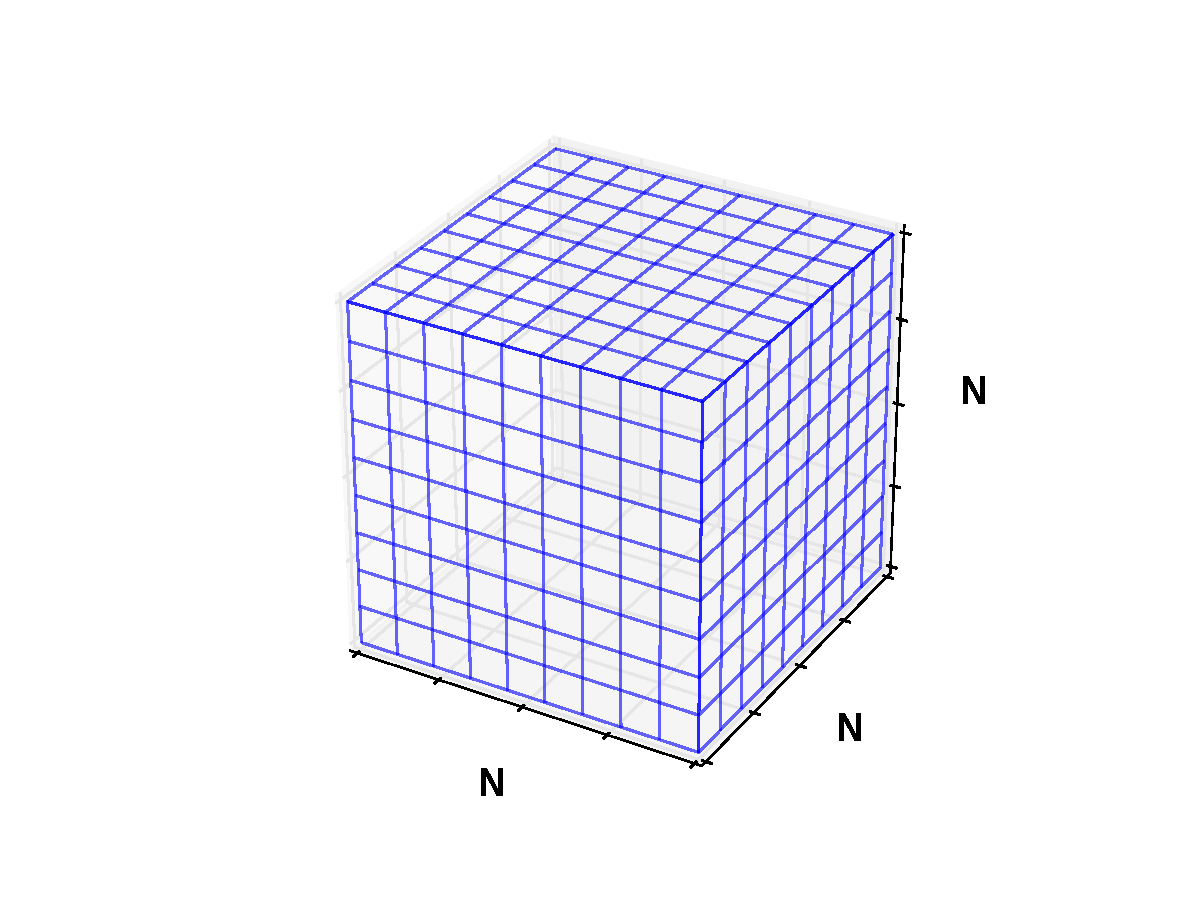
\includegraphics[width=0.4\textwidth]{figures/cube-discretization.pdf}
  \end{center}

  %\pause
  \vspace*{-1.0cm}
   \begin{block}{Compute vs. Communication}
  \begin{itemize}
   \item Take $N=512$, so each field consumes 1 GB of GPU RAM
   \item Boundary communication: $2 \times 6 \times N^2$: 31 MB
   %\pause
   \item Time to process field on GPU: 1.4 ms
   %\pause
   \item Time to load ghost data: \textbf{1.9 ms (!!)}
  \end{itemize}
  \end{block}

\end{frame}
